% AER-Article.tex for AEA last revised 22 June 2011
\documentclass[AER]{AEA}

% The mathtime package uses a Times font instead of Computer Modern.
% Uncomment the line below if you wish to use the mathtime package:
%\usepackage[cmbold]{mathtime}
% Note that miktex, by default, configures the mathtime package to use commercial fonts
% which you may not have. If you would like to use mathtime but you are seeing error
% messages about missing fonts (mtex.pfb, mtsy.pfb, or rmtmi.pfb) then please see
% the technical support document at http://www.aeaweb.org/templates/technical_support.pdf
% for instructions on fixing this problem.

% Note: you may use either harvard or natbib (but not both) to provide a wider
% variety of citation commands than latex supports natively. See below.

% Uncomment the next line to use the natbib package with bibtex
\usepackage{natbib}

% Uncomment the next line to use the harvard package with bibtex
%\usepackage[abbr]{harvard}

% This command determines the leading (vertical space between lines) in draft mode
% with 1.5 corresponding to "double" spacing.
\draftSpacing{1.5}

% Pandoc syntax highlighting
\usepackage{color}
\usepackage{fancyvrb}
\newcommand{\VerbBar}{|}
\newcommand{\VERB}{\Verb[commandchars=\\\{\}]}
\DefineVerbatimEnvironment{Highlighting}{Verbatim}{commandchars=\\\{\}}
% Add ',fontsize=\small' for more characters per line
\usepackage{framed}
\definecolor{shadecolor}{RGB}{248,248,248}
\newenvironment{Shaded}{\begin{snugshade}}{\end{snugshade}}
\newcommand{\AlertTok}[1]{\textcolor[rgb]{0.94,0.16,0.16}{#1}}
\newcommand{\AnnotationTok}[1]{\textcolor[rgb]{0.56,0.35,0.01}{\textbf{\textit{#1}}}}
\newcommand{\AttributeTok}[1]{\textcolor[rgb]{0.13,0.29,0.53}{#1}}
\newcommand{\BaseNTok}[1]{\textcolor[rgb]{0.00,0.00,0.81}{#1}}
\newcommand{\BuiltInTok}[1]{#1}
\newcommand{\CharTok}[1]{\textcolor[rgb]{0.31,0.60,0.02}{#1}}
\newcommand{\CommentTok}[1]{\textcolor[rgb]{0.56,0.35,0.01}{\textit{#1}}}
\newcommand{\CommentVarTok}[1]{\textcolor[rgb]{0.56,0.35,0.01}{\textbf{\textit{#1}}}}
\newcommand{\ConstantTok}[1]{\textcolor[rgb]{0.56,0.35,0.01}{#1}}
\newcommand{\ControlFlowTok}[1]{\textcolor[rgb]{0.13,0.29,0.53}{\textbf{#1}}}
\newcommand{\DataTypeTok}[1]{\textcolor[rgb]{0.13,0.29,0.53}{#1}}
\newcommand{\DecValTok}[1]{\textcolor[rgb]{0.00,0.00,0.81}{#1}}
\newcommand{\DocumentationTok}[1]{\textcolor[rgb]{0.56,0.35,0.01}{\textbf{\textit{#1}}}}
\newcommand{\ErrorTok}[1]{\textcolor[rgb]{0.64,0.00,0.00}{\textbf{#1}}}
\newcommand{\ExtensionTok}[1]{#1}
\newcommand{\FloatTok}[1]{\textcolor[rgb]{0.00,0.00,0.81}{#1}}
\newcommand{\FunctionTok}[1]{\textcolor[rgb]{0.13,0.29,0.53}{\textbf{#1}}}
\newcommand{\ImportTok}[1]{#1}
\newcommand{\InformationTok}[1]{\textcolor[rgb]{0.56,0.35,0.01}{\textbf{\textit{#1}}}}
\newcommand{\KeywordTok}[1]{\textcolor[rgb]{0.13,0.29,0.53}{\textbf{#1}}}
\newcommand{\NormalTok}[1]{#1}
\newcommand{\OperatorTok}[1]{\textcolor[rgb]{0.81,0.36,0.00}{\textbf{#1}}}
\newcommand{\OtherTok}[1]{\textcolor[rgb]{0.56,0.35,0.01}{#1}}
\newcommand{\PreprocessorTok}[1]{\textcolor[rgb]{0.56,0.35,0.01}{\textit{#1}}}
\newcommand{\RegionMarkerTok}[1]{#1}
\newcommand{\SpecialCharTok}[1]{\textcolor[rgb]{0.81,0.36,0.00}{\textbf{#1}}}
\newcommand{\SpecialStringTok}[1]{\textcolor[rgb]{0.31,0.60,0.02}{#1}}
\newcommand{\StringTok}[1]{\textcolor[rgb]{0.31,0.60,0.02}{#1}}
\newcommand{\VariableTok}[1]{\textcolor[rgb]{0.00,0.00,0.00}{#1}}
\newcommand{\VerbatimStringTok}[1]{\textcolor[rgb]{0.31,0.60,0.02}{#1}}
\newcommand{\WarningTok}[1]{\textcolor[rgb]{0.56,0.35,0.01}{\textbf{\textit{#1}}}}

% tightlist command for lists without linebreak
\providecommand{\tightlist}{%
  \setlength{\itemsep}{0pt}\setlength{\parskip}{0pt}}



\usepackage{graphicx}
\usepackage{booktabs}

\usepackage{hyperref}

\begin{document}


\title{Global \(CO_{2}\) Emissions in 1997}
\shortTitle{What Keeling missed all these years}
% \author{Author1 and Author2\thanks{Surname1: affiliation1, address1, email1.
% Surname2: affiliation2, address2, email2. Acknowledgements}}


\author{
  Majid Maki-Nayeri\\
  Vinod Bakthavachalam\\
  Artem Lebedev\thanks{
  Maki-Nayeri: UC Berkeley, School of
Information, \href{mailto:m\_maki@ischool.berkeley.edu}{m\_maki@ischool.berkeley.edu}.
  Bakthavachalam: UC Berkeley, School of
Information, \href{mailto:vinodb@ischool.berkeley.edu}{vinodb@ischool.berkeley.edu}.
  Lebedev: McMaster University, Department of Chemistry and
Biochemistry, \href{mailto:artem.lebedev@berkeley.edu}{artem.lebedev@berkeley.edu}.
  The authors would like to thank their instructors from MIDS 271.
}
}

\date{\today}
\pubMonth{07}
\pubYear{2023}
\pubVolume{0}
\pubIssue{0}
\JEL{}
\Keywords{Replication, Modern Science}

\begin{abstract}
One of the very interesting features of Keeling and colleagues' research
is that they were able to evaluate, and re-evaluate the data as new
series of measurements were released. This permitted the evaluation of
previous models' performance and a much more difficult question: If
their models' predictions were ``off'' was this the result of a failure
of the model, or a change in the system?
\end{abstract}


\maketitle

\hypertarget{introduction}{%
\section{Introduction}\label{introduction}}

\textcolor{red}{In this introduction, you can assume that your reader will have just read your 1997 report. In this introduc-
tion, very briefly pose the question that you are evaluating, and describe what (if anything) has changed in
the data generating process between 1997 and the present.}

\hypertarget{mona-loa-co_2-data}{%
\section{\texorpdfstring{Mona Loa \(CO_{2}\)
Data}{Mona Loa CO\_\{2\} Data}}\label{mona-loa-co_2-data}}

The most current data is provided by the United States' National Oceanic
and Atmospheric Administration, on a data page
{[}\href{https://gml.noaa.gov/ccgg/trends/data.html}{here}{]}. Gather
the most recent weekly data from this page. (A group that is interested
in even more data management might choose to work with the
\href{https://gml.noaa.gov/aftp/data/trace_gases/co2/in-situ/surface/mlo/co2_mlo_surface-insitu_1_ccgg_HourlyData.txt}{hourly
data}.)

Create a data pipeline that starts by reading from the appropriate URL,
and ends by saving an object called \texttt{co2\_present} that is a
suitable time series object.

\hypertarget{recent-trends-in-atmospheric-carbon}{%
\subsection{Recent Trends in Atmospheric
Carbon}\label{recent-trends-in-atmospheric-carbon}}

Conduct the same EDA on this data. Describe how the Keeling Curve
evolved from 1997 to the present, noting where the series seems to be
following similar trends to the series that you ``evaluated in 1997''
and where the series seems to be following different trends. This EDA
can use the same, or very similar tools and views as you provided in
your 1997 report.

\textcolor{red}{Atmospheric carbon is plotted in \autoref{fig:carbon}, and shows some worrying trends. Just look at how wobbly that line is. How is it possible that we are not living in a simulation, when the lines that plots monthly average $CO_{2}$ looks like this?}

\begin{figure}
  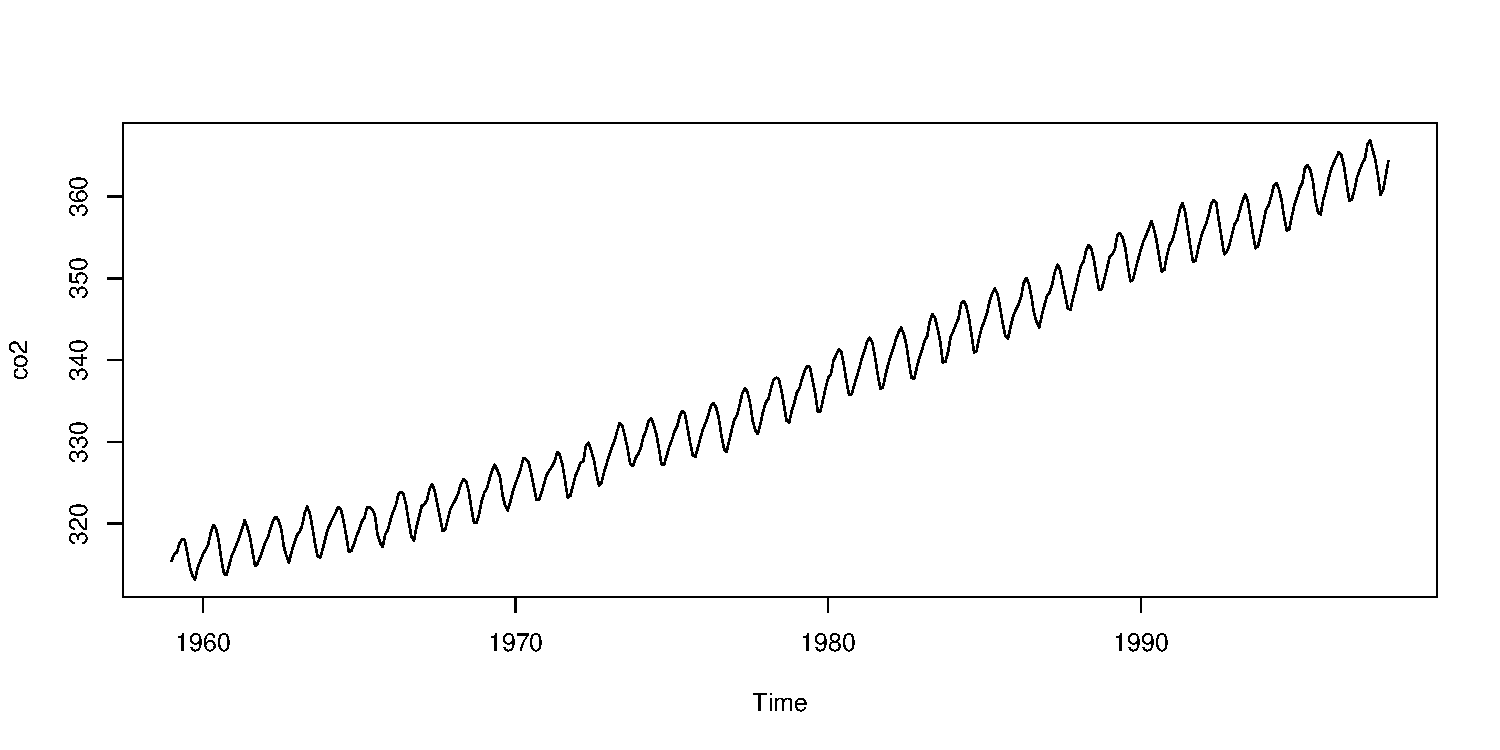
\includegraphics[width=.8\linewidth]{./figures/plot_1.pdf}
  \caption{An uncareful plot.\label{fig:carbon}}
  \begin{figurenotes}
    After giving a declarative statement about what is in the plot, it is useful to provide a very concise interpretation of what you see, or how you read the plot. It should be possible for a reader to \textit{almost} read your entire report from tables, figures, and estimated models.
  \end{figurenotes}
\end{figure}

\textcolor{red}{Even more, a careful examination of \autoref{tab:table_1} suggests some worrying trends in headings and columns. }

\begin{table}
  \caption{What is happening with headers?\label{tab:table_1}}
  \begin{tabular}{lll}
    \toprule 
    & Heading 1 & Heading 2 \\
    Row 1 & 1 & 2 \\
    Row 2 & 3 & 4 \\
    \bottomrule
  \end{tabular}
  \begin{tablenotes}
    Table notes environment without optional leadin.
  \end{tablenotes}
\end{table}

\hypertarget{models-and-forecasts}{%
\section{Models and Forecasts}\label{models-and-forecasts}}

\textcolor{red}{While these plots might be compelling, it is often challenging to learn the exact nature of a time serires process from only these overview, "time vs. outcome" style of plots. In this section, we present evaluate two classes models to assess which time series model is most appropriate to use. }

\hypertarget{linear-models}{%
\subsection{Linear Models}\label{linear-models}}

\textcolor{red}{Descriptively compare realized atmospheric CO2 levels to those predicted by your forecast from a linear time model in 1997 (i.e. "Task 2a"). (You do not need to run any formal tests for this task.) }

\begin{equation}
\label{eq:one}
\text{CO}_{2} = \phi_{0} + \phi_{1} + \epsilon_{eit}
\end{equation}

We estimate best fitting parameters on this model in the following way,

\begin{Shaded}
\begin{Highlighting}[]
\NormalTok{model\_1 }\OtherTok{\textless{}{-}} \FunctionTok{lm}\NormalTok{(y }\SpecialCharTok{\textasciitilde{}}\NormalTok{ x, }\AttributeTok{data =}\NormalTok{ d)}
\end{Highlighting}
\end{Shaded}

\hypertarget{arima-models}{%
\subsection{ARIMA Models}\label{arima-models}}

\textcolor{red}{Descriptively compare realized atmospheric CO2 levels to those predicted by your forecast from the ARIMA model that you fitted in 1997 (i.e. "Task 3a"). Describe how the Keeling Curve evolved from 1997 to the present.}

\hypertarget{performance-of-1997-linear-and-arima-models}{%
\subsection{Performance of 1997 linear and ARIMA
models}\label{performance-of-1997-linear-and-arima-models}}

\textcolor{red}{In 1997 you made predictions about the first time that CO2 would cross 420 ppm. How close were your models to the truth?}

\textcolor{red}{After reflecting on your performance on this threshold-prediction task, continue to use the weekly data to generate a month-average series from 1997 to the present, and compare the overall forecasting performance of your models from Parts 2a and 3b over the entire period. (You should conduct formal tests for this task.)}

\hypertarget{best-models-on-present-data}{%
\subsection{Best models on present
data}\label{best-models-on-present-data}}

\textcolor{red}{Seasonally adjust the weekly NOAA data, and split both seasonally-adjusted (SA) and non-seasonally-adjusted (NSA) series into training and test sets, using the last two years of observations as the test sets. For both SA and NSA series, fit ARIMA models using all appropriate steps. Measure and discuss how your models perform in-sample and (psuedo-) out-of-sample, comparing candidate models and explaining your choice. In addition, fit a polynomial time-trend model to the seasonally-adjusted series and compare its performance to that of your ARIMA model.}

\hypertarget{forecasts-how-bad-could-it-get}{%
\subsection{Forecasts: How bad could it
get?}\label{forecasts-how-bad-could-it-get}}

\textcolor{red}{With the non-seasonally adjusted data series, generate predictions for when atmospheric CO2 is expected to be at 420 ppm and 500 ppm levels for the first and final times (consider prediction intervals as well as point estimates in your answer). Generate a prediction for atmospheric CO2 levels in the year 2122. How confident are you that these will be accurate predictions?}

\textcolor{red}{Because we have fitted a model, we can make predictions from that model. Our preferred model, named in \autoref{eq:one} is quite simple, and as you might notice, does not in fact match up with the model that we have fitted. However, from this model is is possible to reason about what the outcomes would be if the *input concept* were to be slightly ouside of the observed data range. In particular, if *input concept* were as high as $11$, then we would expect the *output concept* to be 10.598, with a prediction interval that ranges from [8.204, 12.992]}\}

\hypertarget{conclusions}{%
\section{Conclusions}\label{conclusions}}

\textcolor{red}{What to conclude is unclear. }

\bibliographystyle{aea}
\bibliography{references}

\appendix
\section{Appendix: Model Robustness}

\textcolor{red}{While the most plausible model that we estimate is reported in the main, "Modeling" section, in this appendix to the article we examine alternative models. Here, our intent is to provide a skeptic that does not accept our assessment of this model as an ARIMA of order (1,2,3) an understanding of model forecasts under alternative scenarios. }


\end{document}
